\documentclass[../Dissertation.tex]{subfiles}

\begin{document}
\section{Evaluation of experimental design}
\textbf{\color{red}
\begin{itemize}
    \item clear result presentation
    \item explain problems and difficulties
    \item demonstrate understanding of results
    \item discuss further work
\end{itemize}
}
\emph{
\begin{itemize}
	\item Duration of training
	\item volume of data gathered
	\item (im)practicalities - power consumption? 
	\item limitations - single optimisation metric
	\item Criticism of methodology
	\item Distiller only supports a single kind of network thinning, so mixing channel and filter pruning was not possible at this time
\end{itemize}
}

\textbf{Challenges}
\begin{itemize}
    \item Very little activity on the distiller repository in the last 6 months
    \item Distiller bugs - distiller shadows the namespace of the standard library python parser module, the path distiller uses to resume a model that has been thinnified is broken - fixed in my fork
    \item onnx issues - must be exported from a checkpoint or retraining doesn't work
\end{itemize}
The size of the pruned networks is not measured.

\subsection{Pipeline Development challenges}
\begin{itemize}
    \item Step 1 | manually prune and retrain with distiller, copy exported model to OpenVino and run the benchmark (baseline and pruned model)
    \item Step 2 | Write code to automate the process from step 1 with hardcoded settings
    \item Step 3 | Create a system to read and write from .yaml files so we can pass in any valid pruning schedule
    \item Step 4 | Integrate this with the wandb sweeps api
\end{itemize}

In order to accomplish Objective~\hyperref[obj:VerifyComp]{O0} before building the pipeline we manually ran each discrete part of the system (Distiller, and OpenVino). 
This immediately highlighted a critical issue; Distiller by default only zeros out the weights when pruning, it doesn't actually remove them from the model so unless a special flag is used with Distiller called `thinnify' there is no measurable benefit to pruning, this issue is exacerbated by the fact that not all pruning algorithms have been implemented to work with `thinnify' and there is little to no documentation on which are compatible. 
A trial and error approach was taken to find pruning algorithms with a working implementation of `thinnify', we systematically tested each of the pruning algorithms that used coarse grained pruning and eventually identified the algorithm described in Section~\ref{sec:FilterPruningAlgo} as fully functional with `thinnify'.

Once we had a verifiable improvement in latency from the baseline metrics described in Section~\ref{sec:baselineData}, we proceeded to develop the pipeline according to Objective~\hyperref[obj:BuildPipeline]{O2}.
Setting up the benchmarking and model queue was very straight forward, for the queue we simply pulled down a docker image of Redis and ran it.
The OpenVino benchmarking tool was very easy to integrate into the pipeline, we simply cleared and then wrote the relevant arguments to \texttt{sys.argv} (pythons array of command line arguments) and called the main method of the benchmarking tool inside OpenVino and captured the output.




\subsection{Hardware and Software}
All agents used in this pipeline used Ubuntu 20.04, we used various hardware configurations for the pruning and retraining agents. 
The benchmarking system was fixed for the duration of the project; a KVM virtual machine, 4 cores/8 threads from a Ryzen 3960X, 8Gb RAM, and the Intel Neural Compute Stick was plugged into a usb controller that was passed through to the VM.
Originally the benchmarking system was combined with the producer system, however due to library and python version compatibility issues we had to run OpenVino and Distiller independently this naturally led us to split the system into agents (Producer \& Consumer).

\textbf{Prune \& retraining software}
\begin{itemize}
    \item Python 3.7.10
    \item Distiller | A python package for neural network compression research
    \item wandb | Weights and biases logging library
    \item PyYaml | Tools to read and write .yaml files
    \item Watchdog | Monitoring of file system events
    \item Redis-py | A python interface to a Redis server
\end{itemize}

\textbf{Benchmarking software}
\begin{itemize}
    \item Python 3.8.5
    \item OpenVino | Deep neural network deployment toolkit
    \item Pandas | Data analysis tool
    \item Redis-py | A python interface to a Redis server
\end{itemize}



\section{Evaluation of results}
\emph{
\begin{itemize}
	\item Summary of results per model/dataset
	\item Deep dive into results, detailed visualisations of accuracy \& latency trade-offs (maybe example with poor quality sensitivity analysis vs higher quality layer selection)
\end{itemize}
}


\subsection{Experiment 1: Rapid pruning}\label{sec:FastPruningPhase}

\begin{figure}[H]
    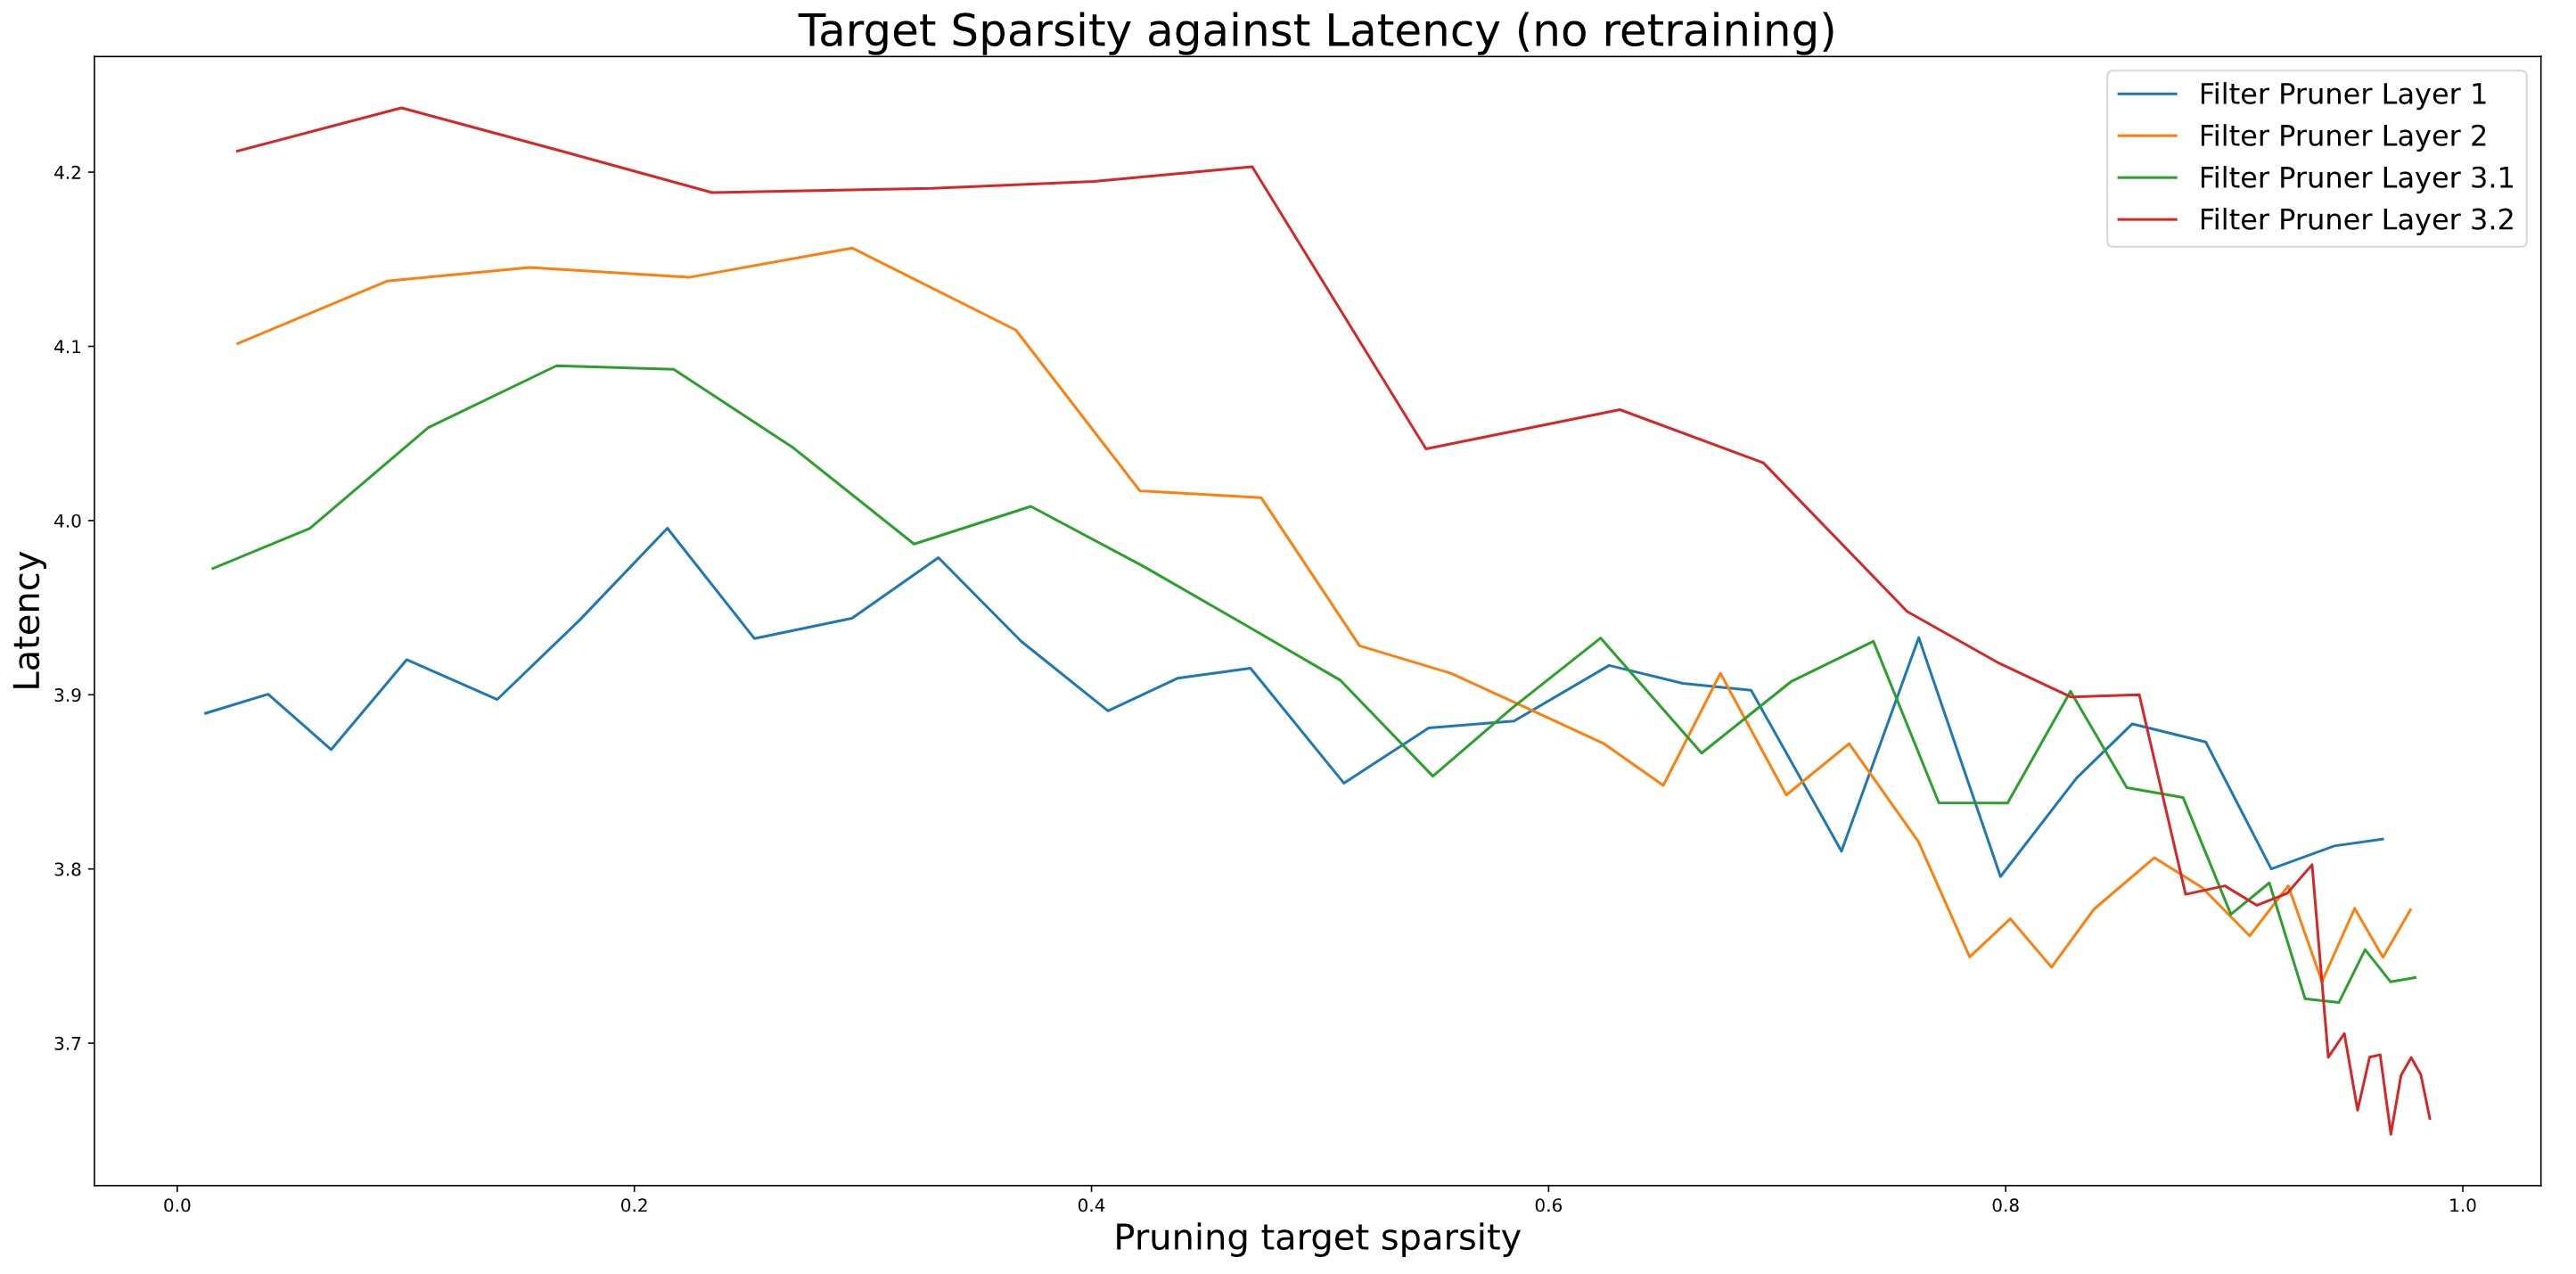
\includegraphics[width=1\textwidth]{TargetSparsityVsLatency_No_Retrain.jpg}
    \caption{Each pruner target sparsity plotted against mean Latency per bin.}
    \label{fig:fastPruneParamVSLatency}
\end{figure}

As discussed in section~\ref{sec:ex1} for this experiment we set the training epochs to 0 and set the target metric to minimize latency. 
During this phase of the experiment we gathered data to observe how pruning would affect latency, this was useful as an initial proof of concept.
This phase of the experiment was very time efficient, we were able to perform 1631 runs with around 18 hours of compute time; each run usually lasted between 24-55 seconds. 
Figure~\ref{fig:fastPruneParamVSLatency} shows the mean Latency computed by using equal width binning, where each bin represents parameter values inside each discretized 0.02 range between 0.0 and 1.0.
This chart does obfuscate any relationship between the parameters, however we can see how the filter pruner on Layer 3.2 (red) plots a more dramatic change in latency than the Pruner on Layer 1 (blue), this is also supported by computing the correlation between these values, see Table~\ref{tab:fastPruneCorrelations}, where `Filter Pruner Layer 3.2' has a strong negative correlation with Latency indicating that increasing the desired sparsity results in an increased tendency to observe a lower latency than `Filter Pruner Layer 1'.

\singlespacing
\begin{table}[H]
    \centering
    \begin{tabular}{@{}cp{26mm}p{26mm}p{26mm}p{26mm}@{}}
    \toprule
    \textbf{Metric}  & \textbf{Filter Pruner  Layer 1} & \textbf{Filter Pruner Layer 2} & \textbf{Filter Pruner Layer 3.1} & \textbf{Filter Pruner Layer 3.2} \\ \midrule
    \textbf{Latency} & $-0.11259$                        & $-0.552583$                      & $-0.40775$                         & $-0.80726$                         \\
    \textbf{Top1}    & $0.004462$                        & $-0.071923$                      & $-0.104505$                        & $-0.152767$                        \\ \bottomrule
    \end{tabular}
    \caption{Correlations between each target sparsity parameter and the metric being measured.}
    \label{tab:fastPruneCorrelations}
\end{table}
\doublespacing

We found that the degree to which we prune was not at all indicative of the resulting accuracy of the network before retraining, for example we observed networks with low desired sparsity across the board that had a much lower Top1 accuracy, than networks that were pruned with much higher targets (See models~\ref{sec:golden-sweep-523}).
It is interesting to note how weakly the pruning targets correlate with Top1 accuracy, this indicates that the relationship between accuracy and pruning is more complex than the naïve perception that pruning less has a smaller accuracy impact.
Observation of this weak correlation with Top1 prompted us to begin logging this initial set of metrics in addition to the metrics we logged as described in the Experimental Design Section~\ref{sec:metricsandparams}, we watched this data in the event that some pattern that might be indicative of how well a pruned network can recover accuracy before retraining has begun will emerge.

We were able to identify a case where pruned networks that have a Top1 accuracy of precisely $100 / n$ where $n$ is the number of classes, the network should be pruned again from scratch, our data had no examples of recovery from this condition during retraining.
Due to the stochastic nature of retraining and the pruning algorithm we selected, coupled with the fact that our methodology necessitated changing the pruning parameters each run we were unable to identify any other pattern or relationship between initial pruning metrics and the metrics of successful or high quality retrained networks from the data we gathered. 



\subsection{Experiment 2: Target Latency}

\subsection{Experiment 3: Target Top1}

\textbf{Interesting observations}
\begin{itemize}
    \item The models that lost all predictive power due to overpruning were not the fastest, even when targeting only latency.
    \item The relationship between more pruning and lower latency is not as simple as you get a faster model with fewer tensors
    \item When targeting accuracy we found models with as low latency when targeting latency directly.
    \item When targeting latency we found models with as high accuracy as when targeting accuracy directly.
    \item Surprising to see that retraining reduces the latency also
\end{itemize}

\end{document}